\documentclass{beamer}

\usepackage[utf8]{inputenc} % Language and font encoding
\usepackage[icelandic]{babel}
\usepackage[T1]{fontenc}


\usepackage{tikz}
\usepackage[listings,theorems]{tcolorbox}
\usepackage{booktabs}
\usepackage{minted} %Minted and configuration
\usemintedstyle{default}

\renewcommand{\theFancyVerbLine}{\sffamily \arabic{FancyVerbLine}}
%%%%%%%%%%%
% More math
%%%%%%%%%%%
\newcommand{\Mod}[1]{\ \text{mod}\ #1}

%%%%%%%%%%%%%%%%%%%%%%
% Beamer configuration
%%%%%%%%%%%%%%%%%%%%%%
\setbeamertemplate{navigation symbols}{}
\usecolortheme{dove}
\setbeamercolor{frametitle}{fg=white}

\usebackgroundtemplate%
{%
\vbox to \paperheight{

\includegraphics[width=\paperwidth]{Pics/hi-slide-head-2016}

\vfill
\hspace{0.5cm}
\includegraphics[width=0.3\paperwidth]{Pics/hi-von-logo}
\vspace{0.4cm}
    }%
}

\AtBeginSection[]
{
  \begin{frame}<beamer>
    \frametitle{Yfirlit}
    \tableofcontents[currentsection]
  \end{frame}
}

\setbeamerfont{frametitle}{size=\normalsize}
\addtobeamertemplate{frametitle}{}{\vspace*{0.5cm}}

%%%%%%%%%%%%%%%%%%%%%%%%%
% tcolorbox configuration
%%%%%%%%%%%%%%%%%%%%%%%%%

% Setup from: http://tex.stackexchange.com/a/43329/21638
\tcbset{%
    noparskip,
    colback=gray!10, %background color of the box
    colframe=gray!40, %color of frame and title background
    coltext=black, %color of body text
    coltitle=black, %color of title text 
    fonttitle=\bfseries,
    alerted/.style={coltitle=red, colframe=gray!40},
    example/.style={coltitle=black, colframe=green!20, colback=green!5},
}


%%%%%%%%%%%%%%%%%%%%%%%
% Further configuration
%%%%%%%%%%%%%%%%%%%%%%%
\hypersetup{colorlinks=true,pdfauthor={Eirikur Ernir Thorsteinsson},linkcolor=blue,urlcolor=blue}
\graphicspath{{./Pics/}}

\author{Eiríkur Ernir Þorsteinsson}
\institute{Háskóli Íslands}
\date{Haust 2016}

\title{Stærðfræðimynstur í tölvunarfræði}
\subtitle{Vika 6, seinni fyrirlestur}

\begin{document}

\begin{frame}
\titlepage
\end{frame}


\section{Inngangur}

\begin{frame}{Í síðasta tíma}
\begin{itemize}
 \item Upprifjun á rakningarvenslum
 \item Endurkvæmar skilgreiningar
 \begin{itemize}
  \item Föll
  \item Mengi
 \end{itemize}
\end{itemize}
\end{frame}

\begin{frame}{Áréttun - af hverju virkar þrepun?}
\begin{itemize}
 \item Þrepun er ekki göldrótt!
 \item Í hefðbundnu grunnskrefi þrepunarsönnunar sýnum við að staðhæfing $P(1)$ sé sönn
 \item Við gerum svo ráð fyrir að $P(k)$ sé satt fyrir ótilgreinda jákvæða heiltölu $k$ og sýnum að $P(k) \to P(k+1)$ fyrir allar jákvæðar heiltölur $k$
 \item Þá getum við séð fyrir okkur að $P(n)$ gildi fyrir allar jákvæðar heiltölur $n$
 \begin{itemize}
  \item Af hverju?
  \item $P(1)$ er satt og við vitum að ef $P(1)$ er satt þá er $P(2)$ líka satt
  \item Þá er $P(2)$ satt og við vitum að ef $P(2)$ er satt þá er $P(3)$ líka satt\ldots
 \end{itemize}
 \item Sönnun í bók
\end{itemize}
\end{frame}

\begin{frame}{Áréttun - sterk þrepun}
\begin{itemize}
 \item Sterk þrepun er sönnunaraðferð sem er jafngild ``venjulegri'' þrepun
 \begin{itemize}
  \item Þ.e.a.s. ef hægt er að nota aðra sönnunaraðferðina má nota hina líka
 \end{itemize}
 \item Þá er ekki sýnt fram á að $P(k) \to P(k+1)$, heldur að \[[P(1) \land P(2) \land \ldots \land P(k)] \to P(k+1)\]
 \item Sterka þrepun er betra að nota þegar ljósara er að $[P(1) \land \ldots \land P(k)] \to P(k+1)$ heldur en að einungis $P(k) \to P(k+1)$
\end{itemize}
\end{frame}


\section{Endurkvæm reiknirit}

\begin{frame}{Endurkvæm reiknirit}
\begin{itemize}
 \item Munum að reiknirit er endanleg runa vel skilgreindra aðgerða sem reikna út lausn á skilgreindu vandamáli
 \item Reiknirit hefur inntak, sem lýsir tilviki af vandamálinu sem það leysir
 \item Reiknirit er kallað endurkvæmt ef það leysir vandamálið með því að smætta það niður í smærra tilvik af sama vandamáli
\end{itemize}
\end{frame}

\begin{frame}{Endurkvæmt hrópmerkt}
Hrópmerkt hentar vel til endurkvæms útreiknings.
\begin{center}
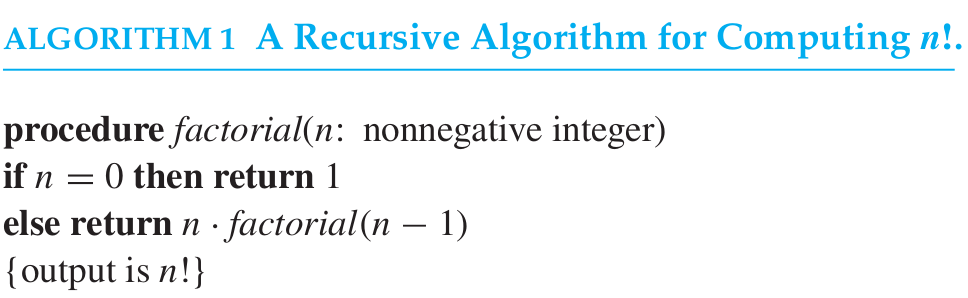
\includegraphics[width=\textwidth]{factorial-algorithm}
\end{center}
\[
3! = 3\cdot 2! = 3 \cdot 2 \cdot 1! = 3 \cdot 2 \cdot 1 \cdot 0! = 3 \cdot 2 \cdot 1 \cdot 1
\]
\end{frame}

\begin{frame}{Endurkvæmt GCD}
\begin{columns}
\column{0.5\textwidth}
Við getum reiknað stærsta samdeili (gcd) með endurkvæmu reikniriti sem byggir á því að 
\[
 gcd(a,b) = gcd(b \Mod a, a)
\]
og að 
\[
 gcd(0,b) = b
\]
þegar $b > 0$.
\column{0.5\textwidth}

\vspace{0.5cm}
Þannig getum við reiknað stærsta samdeili 5 og 8:
\begin{align*}
gcd(5,8) &= gcd(8 \Mod 5, 5)\\
&= gcd(3,5)\\
&= gcd(5 \Mod 3, 3)\\
&= gcd(2,3)\\
&= gcd(3 \Mod 2, 2)\\
&= gcd(1,2)\\
&= gcd(2 \Mod 1, 1)\\
&= gcd(0,1)\\
&= 1
\end{align*}

\end{columns}
\end{frame}

\begin{frame}{Endurkvæmt GCD}
Við getum skrifað reiknirit út frá þessari innsýn:
\begin{center}
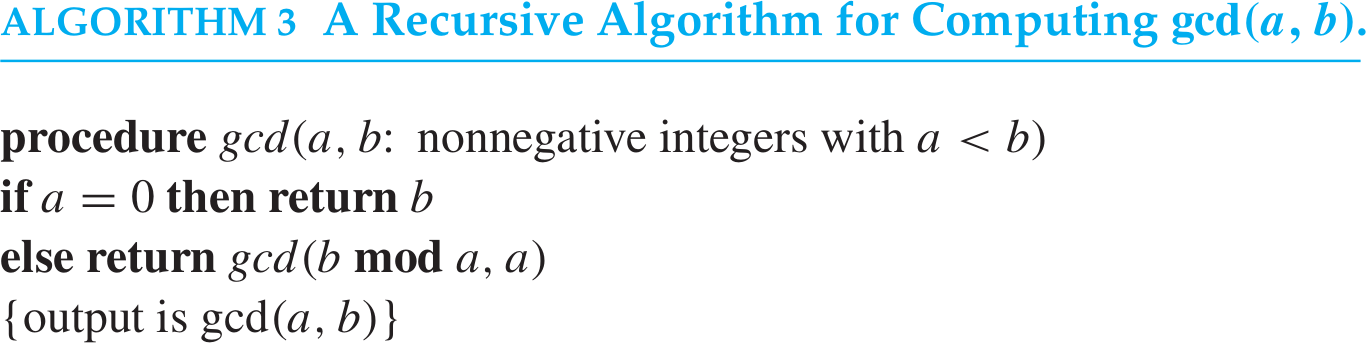
\includegraphics[width=\textwidth]{gcd-recursive}
\end{center}
\end{frame}

\begin{frame}{Línuleg leit}
Rifjum upp línulega leit:
\begin{center}
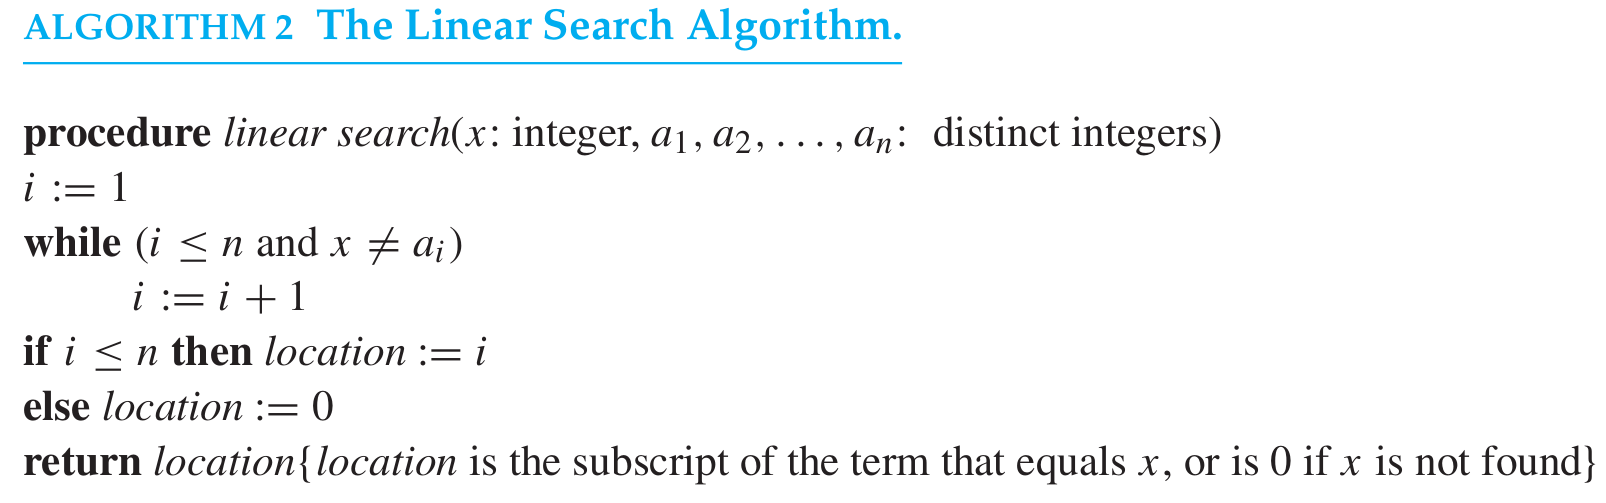
\includegraphics[width=\textwidth]{linear-search}
\end{center}
\end{frame}

\begin{frame}{Endurkvæm línuleg leit?}
Getum við gert endurkvæma útgáfu af línulegri leit?\pause

Já, við getum það:
\begin{center}
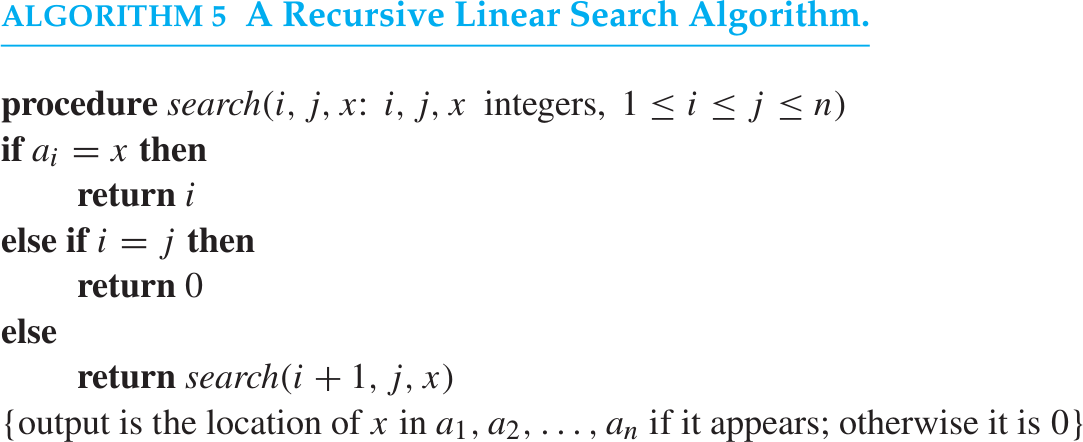
\includegraphics[width=\textwidth]{linear-search-recursive}
\end{center}
\end{frame}

\begin{frame}{Helmingunarleit}
Rifjum upp helmingunarleit:
\begin{center}
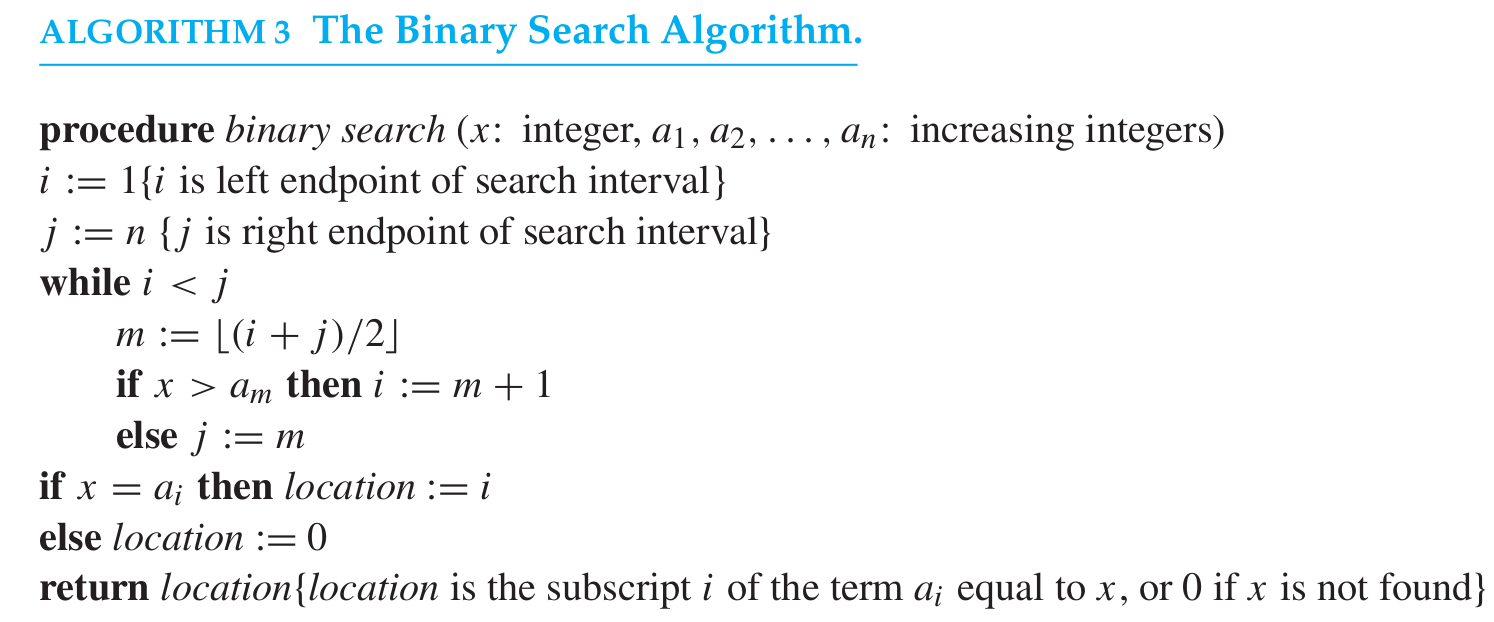
\includegraphics[width=\textwidth]{binary-search}
\end{center}
\end{frame}

\begin{frame}{Endurkvæm helmingunarleit?}
Getum við gert endurkvæma útgáfu af helmingunarleit?\pause

Já, við getum það:
\begin{center}
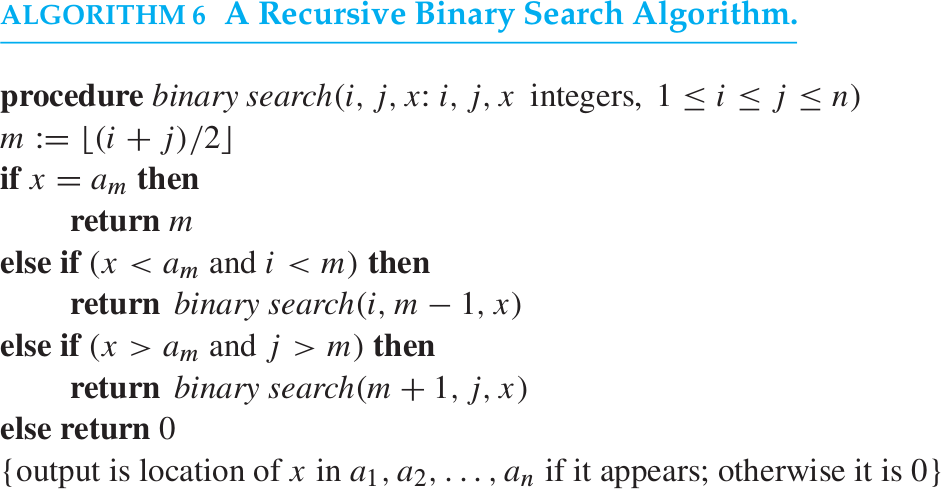
\includegraphics[width=0.8\textwidth]{binary-search-recursive}
\end{center}
\end{frame}

\section{Endurkvæmni og ítrun}

\begin{frame}{Endurkvæmni og ítrun}
\begin{itemize}
 \item Höfum séð endurkvæm reiknirit sem byrja á að skoða heildarmyndina og brjóta hana svo niður í smærri tilvik
 \item Gætum þess í stað séð fyrir okkur að við byrjum á að skoða smáu tilvikin og ``byggjum svo upp'' í þau stóru
 \begin{itemize}
  \item Slíka aðferðafræði köllum við ítrun
  \item Ítrun er venjulega framkvæmd með lykkjum
 \end{itemize}
 \item Ítrun og endurkvæmni framkvæma hliðstæða útreikninga!
\end{itemize}
\end{frame}

\begin{frame}{Endurkvæmni og ítrun}
\begin{itemize}
 \item Hvenær á að nota endurkvæmni og hvenær á að nota ítrun við forritun? \pause
 \begin{itemize}
  \item Ráðlegging undirritaðs: Notið það sem ykkur finnst lýsa vandamálinu best
  \begin{itemize}
   \item Tími forritarans er verðmætur
   \item Getið síðan breytt úr einu í annað ef \emph{mælingar} sýna að upprunalega nálgunin er ekki skilvirk
  \end{itemize}
  \item Þekkið forritunarmálin sem þið eruð að nota - styðja þau endurkvæmni vel?
 \end{itemize}
\end{itemize}
\end{frame}

\section{Merge Sort}

\begin{frame}{Röðun}
\begin{itemize}
 \item Höfum áður séð innsetningarröðun
 \begin{itemize}
  \item Keyrslutími innsetningarröðunar á runu af lengd $n$ er $O(n^2)$ í versta tilfellinu
 \end{itemize}
 \item Skoðum nú endurkvæma lýsingu á reikniriti sem raðar á $O(n\log(n))$ tíma í versta tilfellinu
\end{itemize}
\end{frame}

\begin{frame}{Merge sort}
\begin{itemize}
 \item Hugmyndin að baki merge sort er eftirfarandi:
 \begin{itemize}
  \item Heildarrununni er skipt upp í tvær hlutrunur af jafnri (eða næstum jafnri) lengd
  \begin{itemize}
   \item Hverri hlutrunu er svo skipt upp í tvær hluthlutrunur, o.s.frv.
   \item Uppskiptingunni er haldið áfram þar til runurnar eru af lengdinni 1
  \end{itemize}
  \item Þegar uppskiptingunni er lokið eru runurnar sameinaðar tvær og tvær svo að úr verði röðuð runa
  \begin{itemize}
   \item Þegar síðustu sameiningunni er lokið er runan röðuð!
  \end{itemize}
  \item Merge sort var fundið upp af John von Neumann (1945)
 \end{itemize}
\end{itemize}
\end{frame}

\begin{frame}{Keyrsla merge sort}
\vspace{0.5cm}
\begin{center}
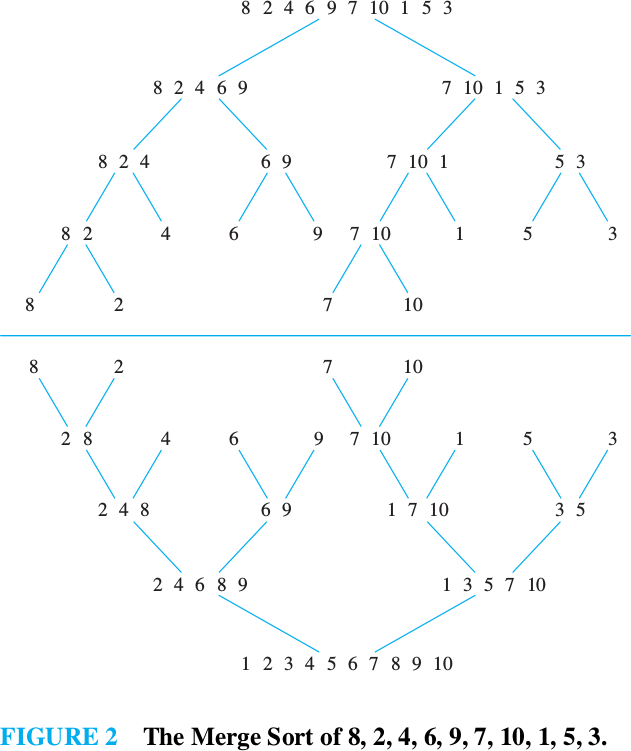
\includegraphics[width=0.5\textwidth]{merge-sort-visual}
\end{center}
\end{frame}

\begin{frame}{Merge reikniritið}
Mikið af vinnunni sem fer fram í merge sort felst í því að sameina listana:
\begin{center}
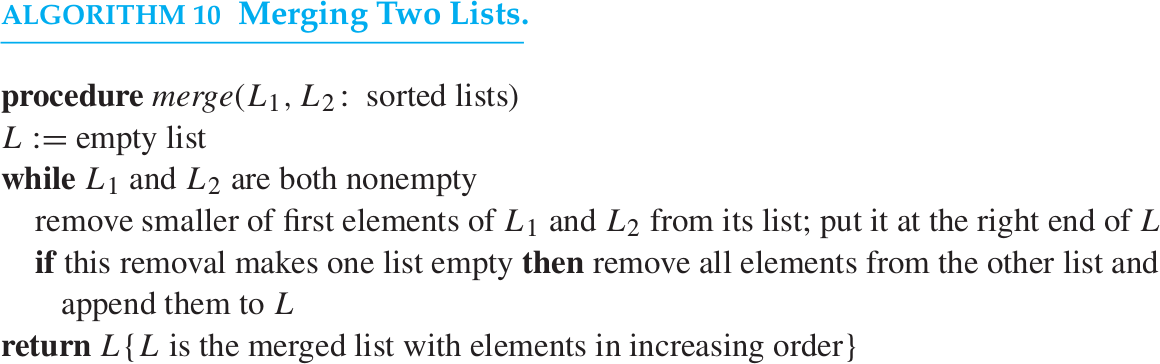
\includegraphics[width=\textwidth]{merge}
\end{center}
\end{frame}

\begin{frame}{Merge sort}
Merge sort er síðan lýst endurkvæmt:
\begin{center}
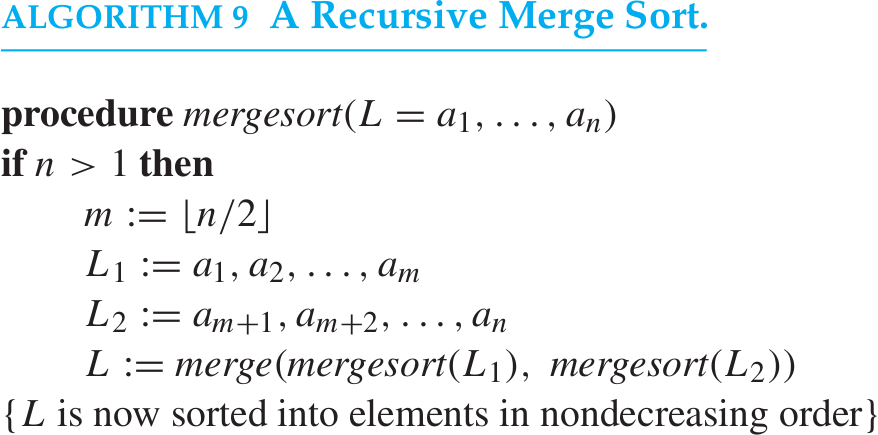
\includegraphics[width=0.9\textwidth]{merge-sort}
\end{center}
\end{frame}

\section{Rökstudd forritun}

\begin{frame}{Rökstudd forritun}
\begin{itemize}
 \item Bókin inniheldur vísi að umfjöllun um rökstudda forritun
 \item Sýnir að hægt er að tengja saman rökfræði og reiknirit
\end{itemize}
\end{frame}

\begin{frame}{Hugtök úr rökstuddri forritun}
\begin{itemize}
 \item Forrit er naumrétt (e. \emph{partially correct} eða \emph{weakly correct}) skili það ``réttri niðurstöðu'' þegar forritið er ``rétt notað'' og lýkur keyrslu
 \item Til skilgreiningar á því hvað teljist rétt eru hugtökin forskilyrði (e. \emph{precondition} eða \emph{initial assertion}) og eftirskilyrði (e. \emph{postcondition} eða \emph{final assertion}) notuð
 \begin{itemize}
  \item Forskilyrði lýsa þeim aðstæðum sem þurfa að gilda áður en forrit keyrir (venjulega lýsing eiginleikum inntaks)
  \item Eftirskilyrði lýsir þeim aðstæðum sem gilda eftir að forrit keyrir (venjulega lýsing á eiginleikum skilagildis)
 \end{itemize}
\end{itemize}
\end{frame}

\begin{frame}{Naumrétt forrit}
\begin{tcolorbox}[title=Naumrétt forrit]
Forrit eða forritsbútur $S$ er naumréttur með tilliti til forskilyrðisins $p$ og eftirskilyrðisins $q$ ef $q$ er satt hvenær sem $p$ er satt og $S$ lýkur keyrslu.

Rithátturinn $p\{S\}q$ táknar að $S$ sé naumrétt með tilliti til forskilyrðisins $p$ og eftirskilyrðisins $q$.
\end{tcolorbox}
Sé forrit naumrétt m.t.t. gefinna skilyrða og auk þess er tryggt að það ljúki alltaf keyrslu við gefin skilyrði er það rammrétt (e. \emph{correct} eða \emph{strongly correct}).

Rithátturinn $p\{S\}q$ er kallaður Hoare þrennd (e. \emph{Hoare triple}).
\end{frame}

\begin{frame}{Rökstutt forrit}
Sýnum að forritsbúturinn
\begin{align*}
y &:= 2\\
z &:= x + y
\end{align*}
sé naumréttur m.t.t. upphafsskilyrðisins $p: x = 1$ og eftirskilyrðisins $q: z = 3$. \pause

G.r.f.a. $p$ sé satt. $y$ fær gildið 2. Þar sem $p$ er satt fær $z$ gildið $1+2 = 3$. Þá er $q$ satt, svo $p\{S\}q$ er satt.
\end{frame}

\begin{frame}{Lengri rökstudd forrit}
\begin{itemize}
 \item Við getum rökstutt lengri forrit með því að brjóta þau niður í rökstudda forritsbúta
 \item Við getum skilgreint leiðir til að rökstyðja forritsbúta sem fela í sér algeng forritunarhugtök:
 \begin{itemize}
  \item Lykkjur
  \item Stýrisetningar
 \end{itemize}
 \item Gildi, fyrir gefna forritsbúta $S_1$ og $S_1$ bæði $p\{S_1\}q$ og $q\{s_2\}r$, þá má fyrir samsetta forritið $S = S_1;S_2$ skrifa $p\{S_1; S_2\}r$ eða einfaldlega $p\{S\}r$
\end{itemize}
\end{frame}


\begin{frame}{Næst}
Talning (6.1) og skúffureglan (6.2)
\end{frame}


\end{document}
